\section{BTB\_\-btac\_\-t Class Reference}
\label{classBTB__btac__t}\index{BTB\_\-btac\_\-t@{BTB\_\-btac\_\-t}}
Inheritance diagram for BTB\_\-btac\_\-t:\nopagebreak
\begin{figure}[H]
\begin{center}
\leavevmode
\includegraphics[height=400pt]{classBTB__btac__t__inherit__graph}
\end{center}
\end{figure}
Collaboration diagram for BTB\_\-btac\_\-t:\nopagebreak
\begin{figure}[H]
\begin{center}
\leavevmode
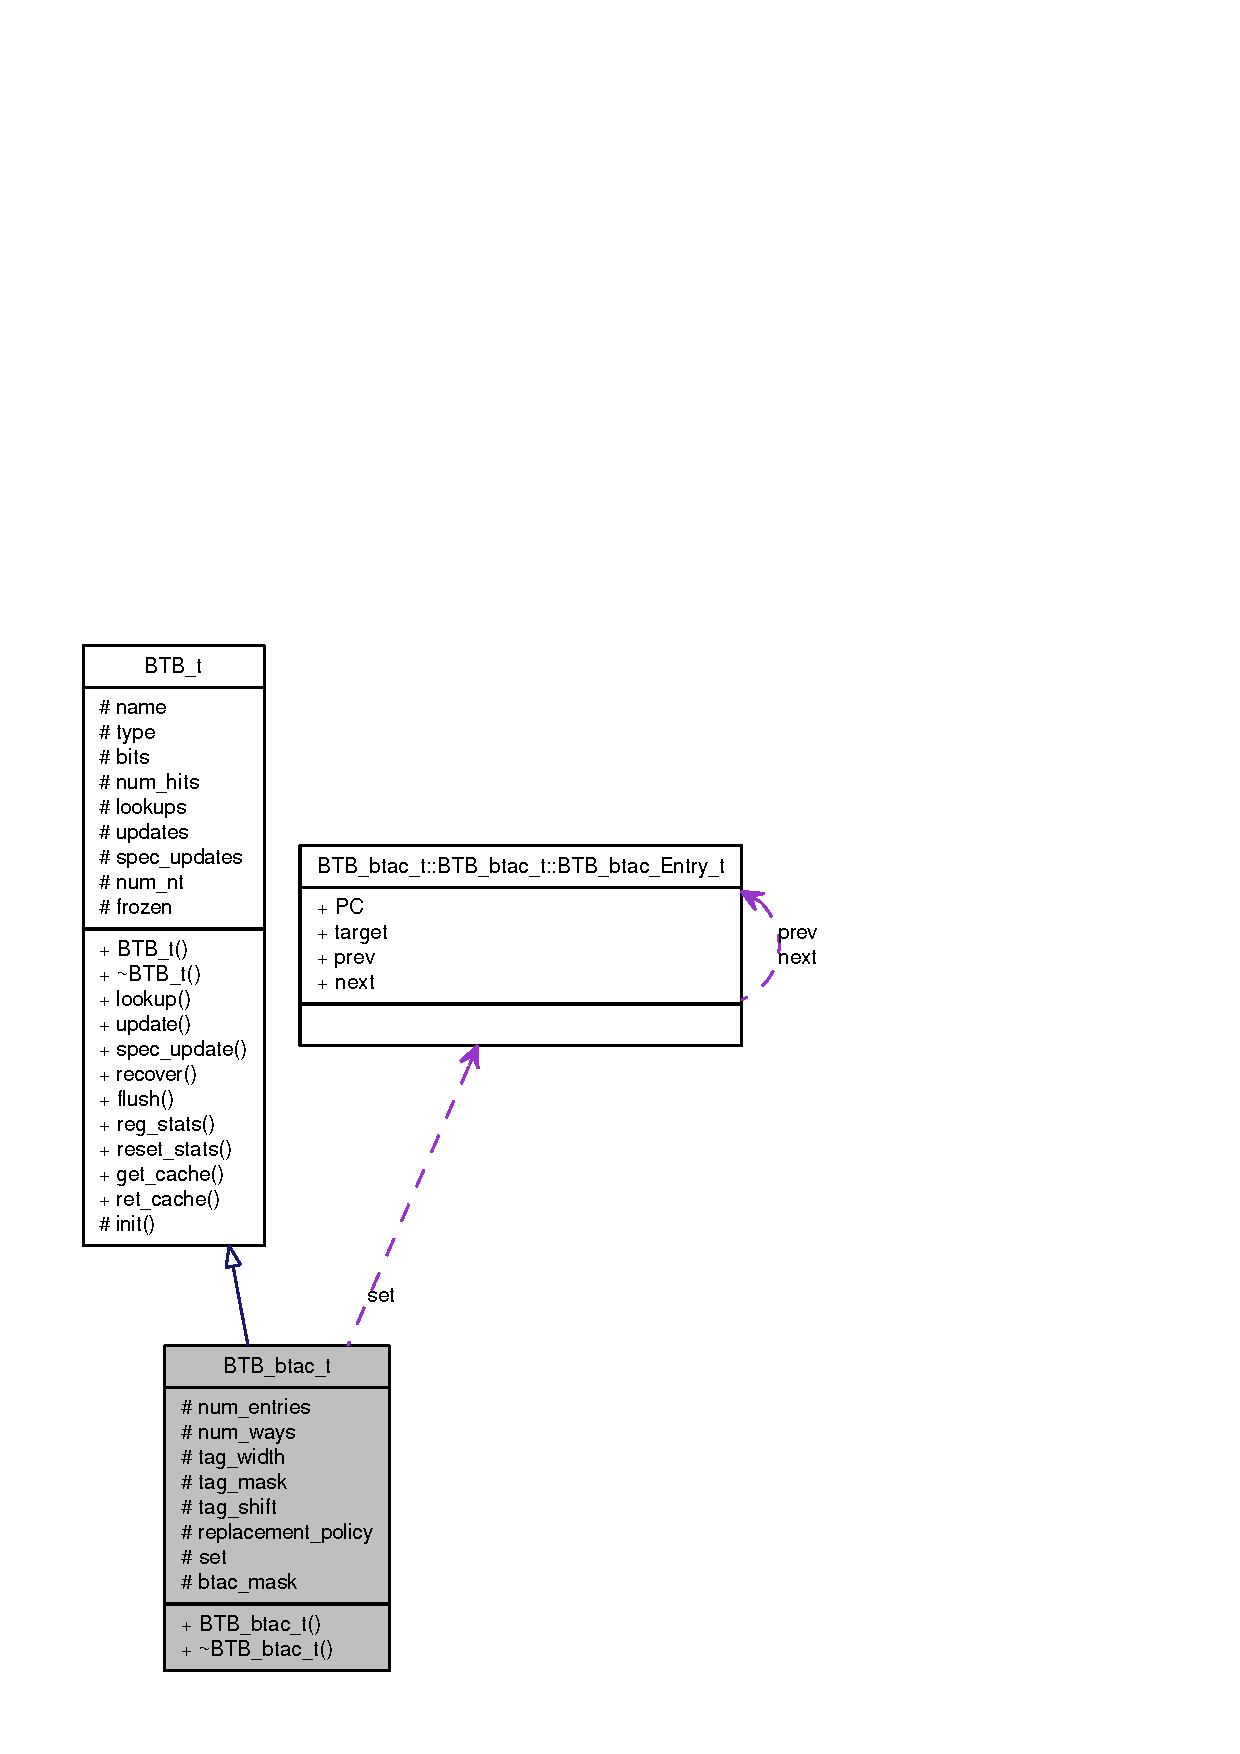
\includegraphics[height=400pt]{classBTB__btac__t__coll__graph}
\end{center}
\end{figure}
\subsection*{Classes}
\begin{CompactItemize}
\item 
struct {\bf BTB\_\-btac\_\-Entry\_\-t}
\item 
class {\bf BTB\_\-btac\_\-sc\_\-t}
\end{CompactItemize}
\subsection*{Public Member Functions}
\begin{CompactItemize}
\item 
{\bf BTB\_\-btac\_\-t} (char $\ast$const arg\_\-name, const int arg\_\-num\_\-entries, const int arg\_\-num\_\-ways, const int arg\_\-tag\_\-width, const char arg\_\-replacement\_\-policy)
\item 
{\bf $\sim$BTB\_\-btac\_\-t} ()
\end{CompactItemize}
\subsection*{Protected Attributes}
\begin{CompactItemize}
\item 
int {\bf num\_\-entries}
\item 
int {\bf num\_\-ways}
\item 
int {\bf tag\_\-width}
\item 
int {\bf tag\_\-mask}
\item 
int {\bf tag\_\-shift}
\item 
char {\bf replacement\_\-policy}
\item 
struct {\bf BTB\_\-btac\_\-Entry\_\-t} $\ast$$\ast$ {\bf set}
\item 
int {\bf btac\_\-mask}
\end{CompactItemize}


\subsection{Detailed Description}


Definition at line 22 of file btb-btac.cpp.

\subsection{Constructor \& Destructor Documentation}
\index{BTB\_\-btac\_\-t@{BTB\_\-btac\_\-t}!BTB\_\-btac\_\-t@{BTB\_\-btac\_\-t}}
\index{BTB\_\-btac\_\-t@{BTB\_\-btac\_\-t}!BTB_btac_t@{BTB\_\-btac\_\-t}}
\subsubsection[{BTB\_\-btac\_\-t}]{\setlength{\rightskip}{0pt plus 5cm}BTB\_\-btac\_\-t::BTB\_\-btac\_\-t (char $\ast$const  {\em arg\_\-name}, \/  const int {\em arg\_\-num\_\-entries}, \/  const int {\em arg\_\-num\_\-ways}, \/  const int {\em arg\_\-tag\_\-width}, \/  const char {\em arg\_\-replacement\_\-policy})\hspace{0.3cm}{\tt  [inline]}}\label{classBTB__btac__t_755509512947df4573ba72ae340e85a5}




Definition at line 53 of file btb-btac.cpp.

References BTB\_\-t::bits, btac\_\-mask, CHECK\_\-POS, CHECK\_\-PPOW2, COMPONENT\_\-NAME, fatal(), BTB\_\-t::init(), log\_\-base2(), mytolower(), BTB\_\-t::name, BTB\_\-btac\_\-t::BTB\_\-btac\_\-t::BTB\_\-btac\_\-Entry\_\-t::next, num\_\-entries, num\_\-ways, BTB\_\-btac\_\-t::BTB\_\-btac\_\-t::BTB\_\-btac\_\-Entry\_\-t::prev, replacement\_\-policy, tag\_\-mask, tag\_\-shift, tag\_\-width, and BTB\_\-t::type.\index{BTB\_\-btac\_\-t@{BTB\_\-btac\_\-t}!$\sim$BTB\_\-btac\_\-t@{$\sim$BTB\_\-btac\_\-t}}
\index{$\sim$BTB\_\-btac\_\-t@{$\sim$BTB\_\-btac\_\-t}!BTB_btac_t@{BTB\_\-btac\_\-t}}
\subsubsection[{$\sim$BTB\_\-btac\_\-t}]{\setlength{\rightskip}{0pt plus 5cm}BTB\_\-btac\_\-t::$\sim$BTB\_\-btac\_\-t ()\hspace{0.3cm}{\tt  [inline]}}\label{classBTB__btac__t_65dcc2cf26ada35a1efa071dcea28b4e}




Definition at line 111 of file btb-btac.cpp.

References BTB\_\-t::name, BTB\_\-btac\_\-t::BTB\_\-btac\_\-t::BTB\_\-btac\_\-Entry\_\-t::next, num\_\-entries, and BTB\_\-t::type.

\subsection{Member Data Documentation}
\index{BTB\_\-btac\_\-t@{BTB\_\-btac\_\-t}!btac\_\-mask@{btac\_\-mask}}
\index{btac\_\-mask@{btac\_\-mask}!BTB_btac_t@{BTB\_\-btac\_\-t}}
\subsubsection[{btac\_\-mask}]{\setlength{\rightskip}{0pt plus 5cm}int {\bf BTB\_\-btac\_\-t::btac\_\-mask}\hspace{0.3cm}{\tt  [protected]}}\label{classBTB__btac__t_4edf7639bee62f9e4fc1484673b7be34}




Definition at line 49 of file btb-btac.cpp.

Referenced by BTB\_\-btac\_\-t().\index{BTB\_\-btac\_\-t@{BTB\_\-btac\_\-t}!num\_\-entries@{num\_\-entries}}
\index{num\_\-entries@{num\_\-entries}!BTB_btac_t@{BTB\_\-btac\_\-t}}
\subsubsection[{num\_\-entries}]{\setlength{\rightskip}{0pt plus 5cm}int {\bf BTB\_\-btac\_\-t::num\_\-entries}\hspace{0.3cm}{\tt  [protected]}}\label{classBTB__btac__t_f9c6785dfbbfe6517e180e09d016e395}




Definition at line 41 of file btb-btac.cpp.

Referenced by BTB\_\-btac\_\-t(), and $\sim$BTB\_\-btac\_\-t().\index{BTB\_\-btac\_\-t@{BTB\_\-btac\_\-t}!num\_\-ways@{num\_\-ways}}
\index{num\_\-ways@{num\_\-ways}!BTB_btac_t@{BTB\_\-btac\_\-t}}
\subsubsection[{num\_\-ways}]{\setlength{\rightskip}{0pt plus 5cm}int {\bf BTB\_\-btac\_\-t::num\_\-ways}\hspace{0.3cm}{\tt  [protected]}}\label{classBTB__btac__t_0f4fff09dba86636a5ac899279f195c3}




Definition at line 42 of file btb-btac.cpp.

Referenced by BTB\_\-btac\_\-t().\index{BTB\_\-btac\_\-t@{BTB\_\-btac\_\-t}!replacement\_\-policy@{replacement\_\-policy}}
\index{replacement\_\-policy@{replacement\_\-policy}!BTB_btac_t@{BTB\_\-btac\_\-t}}
\subsubsection[{replacement\_\-policy}]{\setlength{\rightskip}{0pt plus 5cm}char {\bf BTB\_\-btac\_\-t::replacement\_\-policy}\hspace{0.3cm}{\tt  [protected]}}\label{classBTB__btac__t_7027eff9e17bd92e31c5ed5fd14a5979}




Definition at line 46 of file btb-btac.cpp.

Referenced by BTB\_\-btac\_\-t().\index{BTB\_\-btac\_\-t@{BTB\_\-btac\_\-t}!set@{set}}
\index{set@{set}!BTB_btac_t@{BTB\_\-btac\_\-t}}
\subsubsection[{set}]{\setlength{\rightskip}{0pt plus 5cm}struct {\bf BTB\_\-btac\_\-Entry\_\-t}$\ast$$\ast$ {\bf BTB\_\-btac\_\-t::set}\hspace{0.3cm}{\tt  [read, protected]}}\label{classBTB__btac__t_12d11e918708dc364866fef068d1679b}




Definition at line 47 of file btb-btac.cpp.\index{BTB\_\-btac\_\-t@{BTB\_\-btac\_\-t}!tag\_\-mask@{tag\_\-mask}}
\index{tag\_\-mask@{tag\_\-mask}!BTB_btac_t@{BTB\_\-btac\_\-t}}
\subsubsection[{tag\_\-mask}]{\setlength{\rightskip}{0pt plus 5cm}int {\bf BTB\_\-btac\_\-t::tag\_\-mask}\hspace{0.3cm}{\tt  [protected]}}\label{classBTB__btac__t_d690e1d2bcb7b28373fdf5b067efb173}




Definition at line 44 of file btb-btac.cpp.

Referenced by BTB\_\-btac\_\-t().\index{BTB\_\-btac\_\-t@{BTB\_\-btac\_\-t}!tag\_\-shift@{tag\_\-shift}}
\index{tag\_\-shift@{tag\_\-shift}!BTB_btac_t@{BTB\_\-btac\_\-t}}
\subsubsection[{tag\_\-shift}]{\setlength{\rightskip}{0pt plus 5cm}int {\bf BTB\_\-btac\_\-t::tag\_\-shift}\hspace{0.3cm}{\tt  [protected]}}\label{classBTB__btac__t_a1367f1b164090a6366def5f57deae63}




Definition at line 45 of file btb-btac.cpp.

Referenced by BTB\_\-btac\_\-t().\index{BTB\_\-btac\_\-t@{BTB\_\-btac\_\-t}!tag\_\-width@{tag\_\-width}}
\index{tag\_\-width@{tag\_\-width}!BTB_btac_t@{BTB\_\-btac\_\-t}}
\subsubsection[{tag\_\-width}]{\setlength{\rightskip}{0pt plus 5cm}int {\bf BTB\_\-btac\_\-t::tag\_\-width}\hspace{0.3cm}{\tt  [protected]}}\label{classBTB__btac__t_946f59049044953739a118d4df76fbf2}




Definition at line 43 of file btb-btac.cpp.

Referenced by BTB\_\-btac\_\-t().

The documentation for this class was generated from the following file:\begin{CompactItemize}
\item 
{\bf btb-btac.cpp}\end{CompactItemize}
